\section[NACA0012]{\textbf{NACA0012 Icing Results}}

% ============================================================
% NACA0012 -- ICING RESULTS
% ============================================================

\begin{frame}[plain]
    \centering
    \vfill

    {\LARGE\bfseries NACA0012 RESULTS}

    \vfill
\end{frame}

% ============================================================
% NACA0012 -- Integrated Aerodynamic Coefficients
% ============================================================

\begin{frame}{\small NACA0012 -- Integrated Aerodynamic Coefficients}
\scriptsize

\vspace{-0.1cm}

\begin{columns}[T,onlytextwidth]

% ------------------------------------------------------------
% CL
% ------------------------------------------------------------
\begin{column}{0.33\textwidth}
    \centering
    \textbf{$C_L$}

    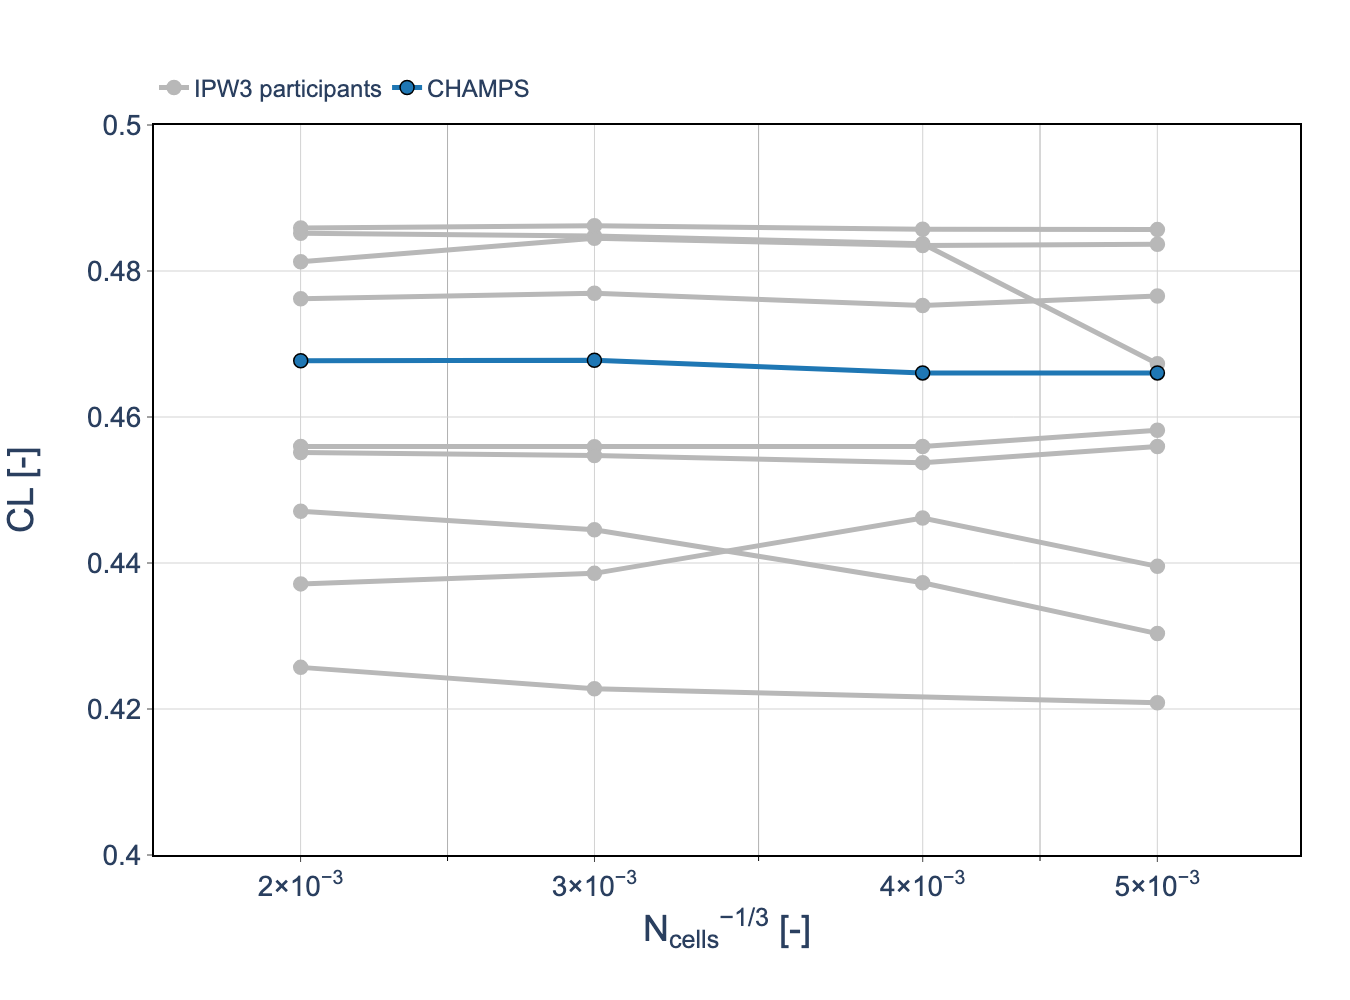
\includegraphics[
        width=\textwidth,
        trim={0cm 0cm 1cm 2.6cm},
        clip
    ]
    {FIGURES/NACA0012/AERODYNAMIC/tc_naca0012_ae3932_cl_vs_n_all_roughness.png}
\end{column}

% ------------------------------------------------------------
% CD
% ------------------------------------------------------------
\begin{column}{0.33\textwidth}
    \centering
    \textbf{$C_D$}

    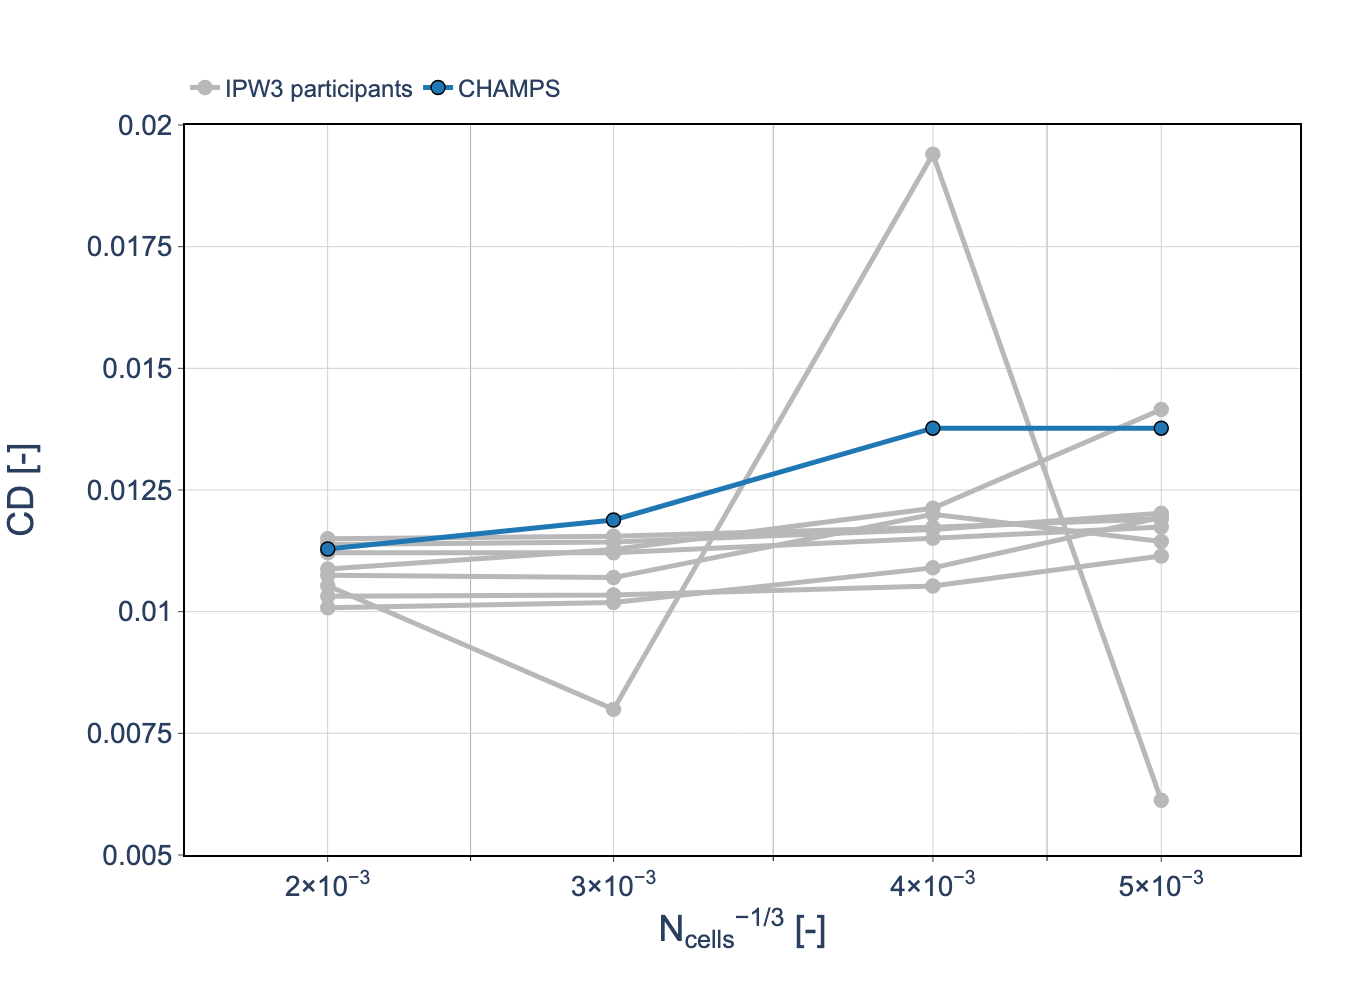
\includegraphics[
        width=\textwidth,
        trim={0cm 0cm 1cm 2.6cm},
        clip
    ]
    {FIGURES/NACA0012/AERODYNAMIC/tc_naca0012_ae3932_cd_vs_n_all_roughness.png}
\end{column}

% ------------------------------------------------------------
% CM
% ------------------------------------------------------------
\begin{column}{0.33\textwidth}
    \centering
    \textbf{$C_M$}

    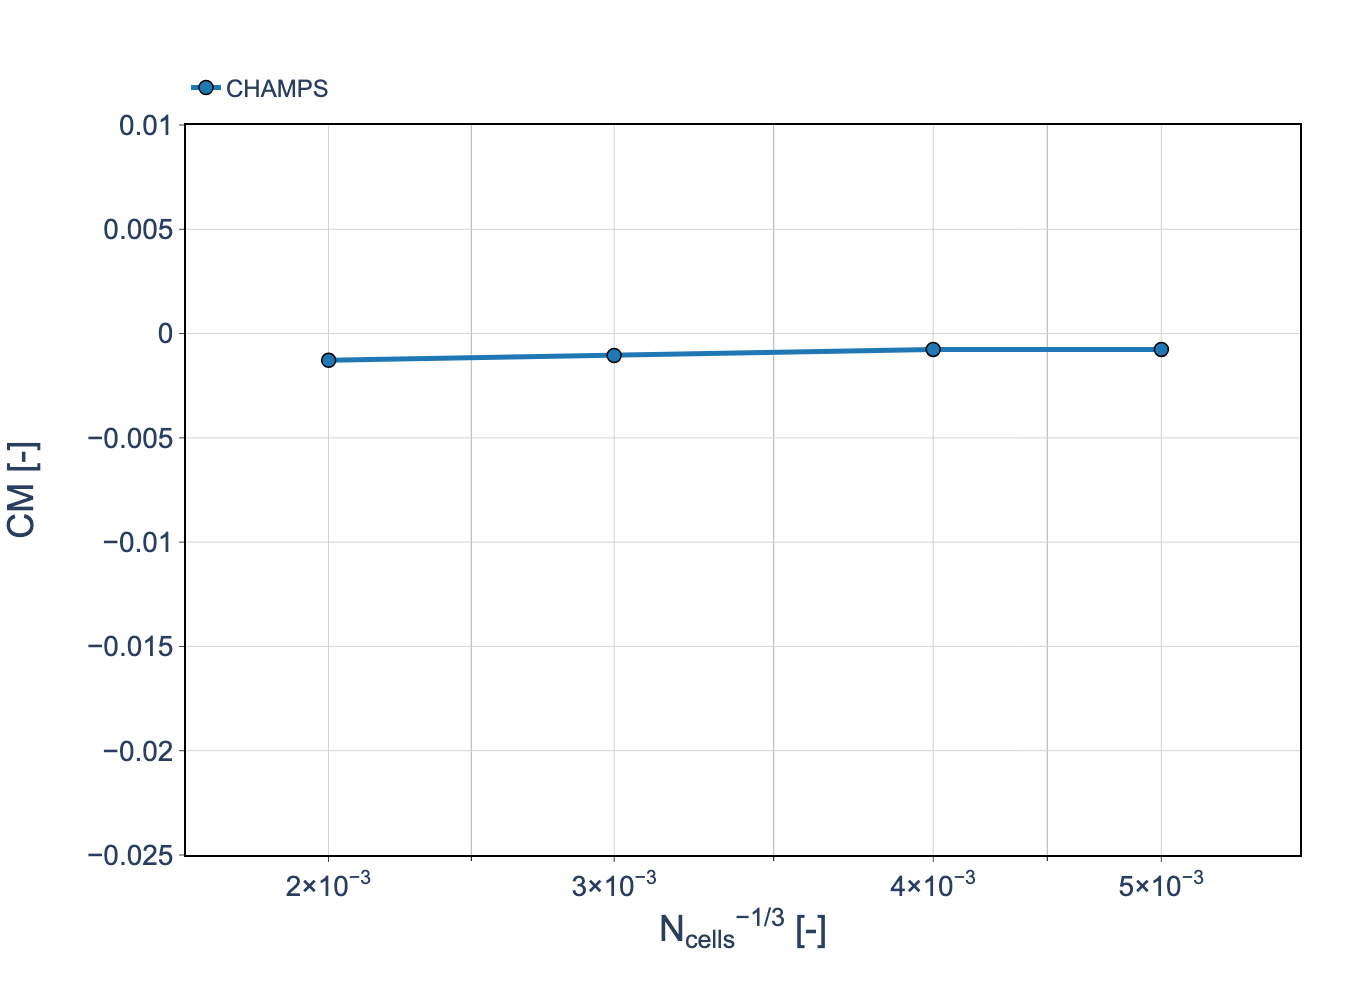
\includegraphics[
        width=\textwidth,
        trim={0cm 0cm 1cm 2.6cm},
        clip
    ]
    {FIGURES/NACA0012/AERODYNAMIC/tc_naca0012_ae3932_cmy_vs_n_all_roughness.png}
\end{column}

\end{columns}

\vspace{-0.10cm}

\begin{center}
\renewcommand{\arraystretch}{1.20}
\setlength{\tabcolsep}{6pt}

\begin{tabular}{lccc}
\toprule
& $\mathbf{C_L}$ & $\mathbf{C_D}$ & $\mathbf{C_M}$ \\
\midrule

\textbf{CHAMPS}
& 0.4677
& 0.01129
& -0.00128 \\

\textbf{IPW3 L1 Median}
& 0.4657
& 0.01088
& -0.00295 \\

\textbf{Difference}
& +0.43\%
& +3.77\%
& +0.00167 \\

\bottomrule
\end{tabular}
\end{center}

\vspace{-0.15cm}

\begin{block}{\scriptsize Integrated Aerodynamic Coefficients Assessment}
CHAMPS predicts integrated aerodynamic coefficients close to the IPW3 L1
median. $C_D$ exhibits the greatest sensitivity to spatial grid refinement.
\end{block}

\end{frame}


% ============================================================
% NACA0012 -- Pressure Distribution
% ============================================================

\begin{frame}{\small NACA0012 -- Pressure-Coefficient Distribution}
\scriptsize

\vspace{-0.15cm}

\begin{columns}[T,onlytextwidth]

% ------------------------------------------------------------
% Cp vs x
% ------------------------------------------------------------
\begin{column}{0.50\textwidth}
    \centering
    \textbf{$C_p$ vs. $x$}

    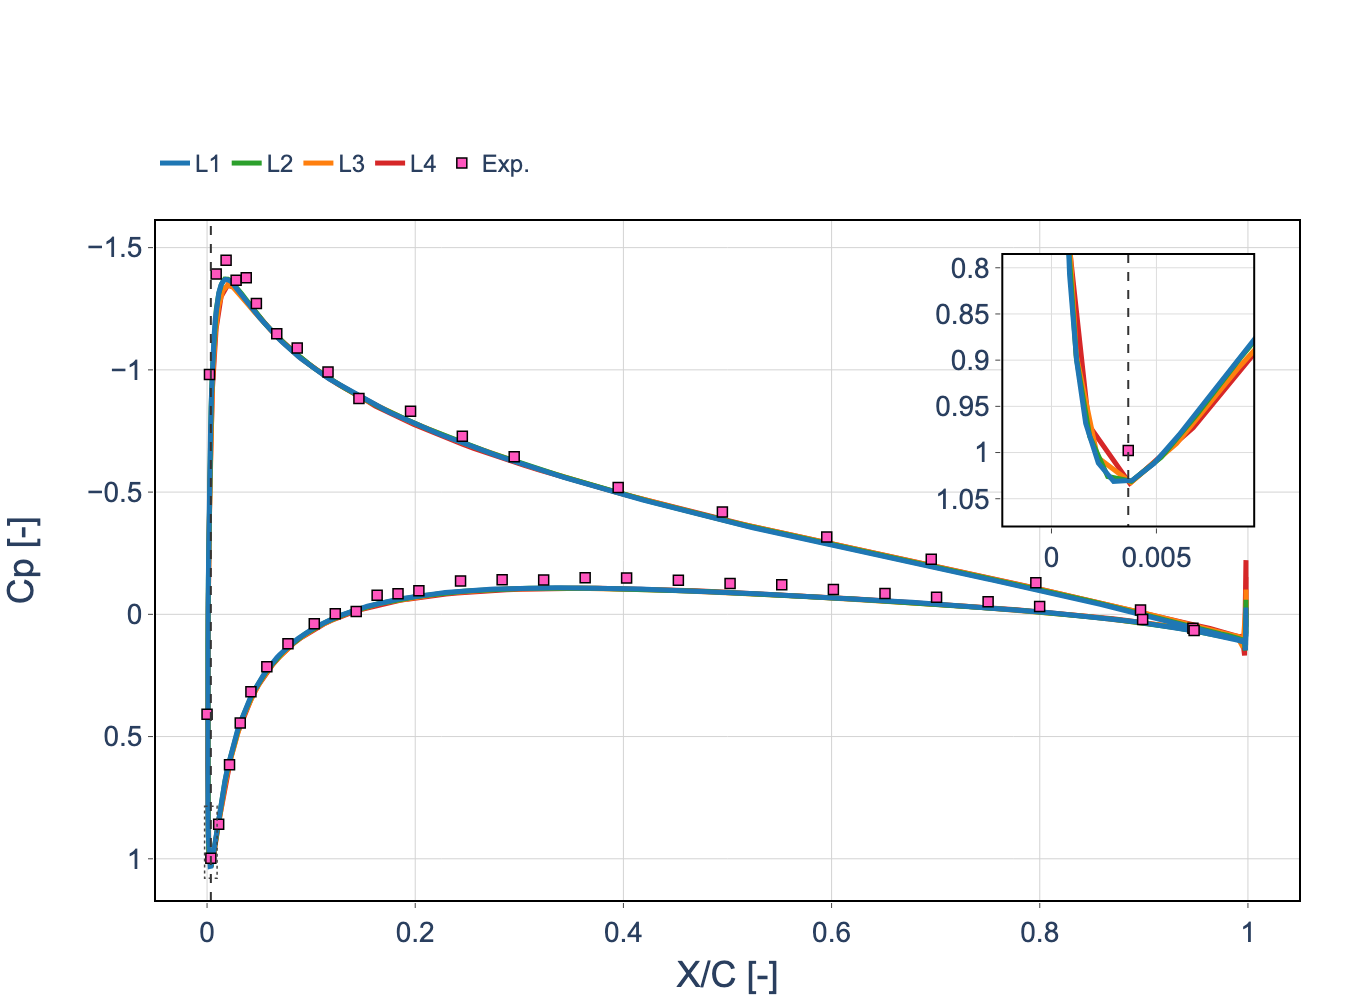
\includegraphics[
        width=\textwidth,
        trim={0cm 0cm 1cm 3.0cm},
        clip
    ]
    {FIGURES/NACA0012/AERODYNAMIC/tc_naca0012_ae3932_L1_cp_vs_x_slice_0p9144_all_roughness.png}
\end{column}

% ------------------------------------------------------------
% Cp vs s
% ------------------------------------------------------------
\begin{column}{0.50\textwidth}
    \centering
    \textbf{$C_p$ vs. $s$}

    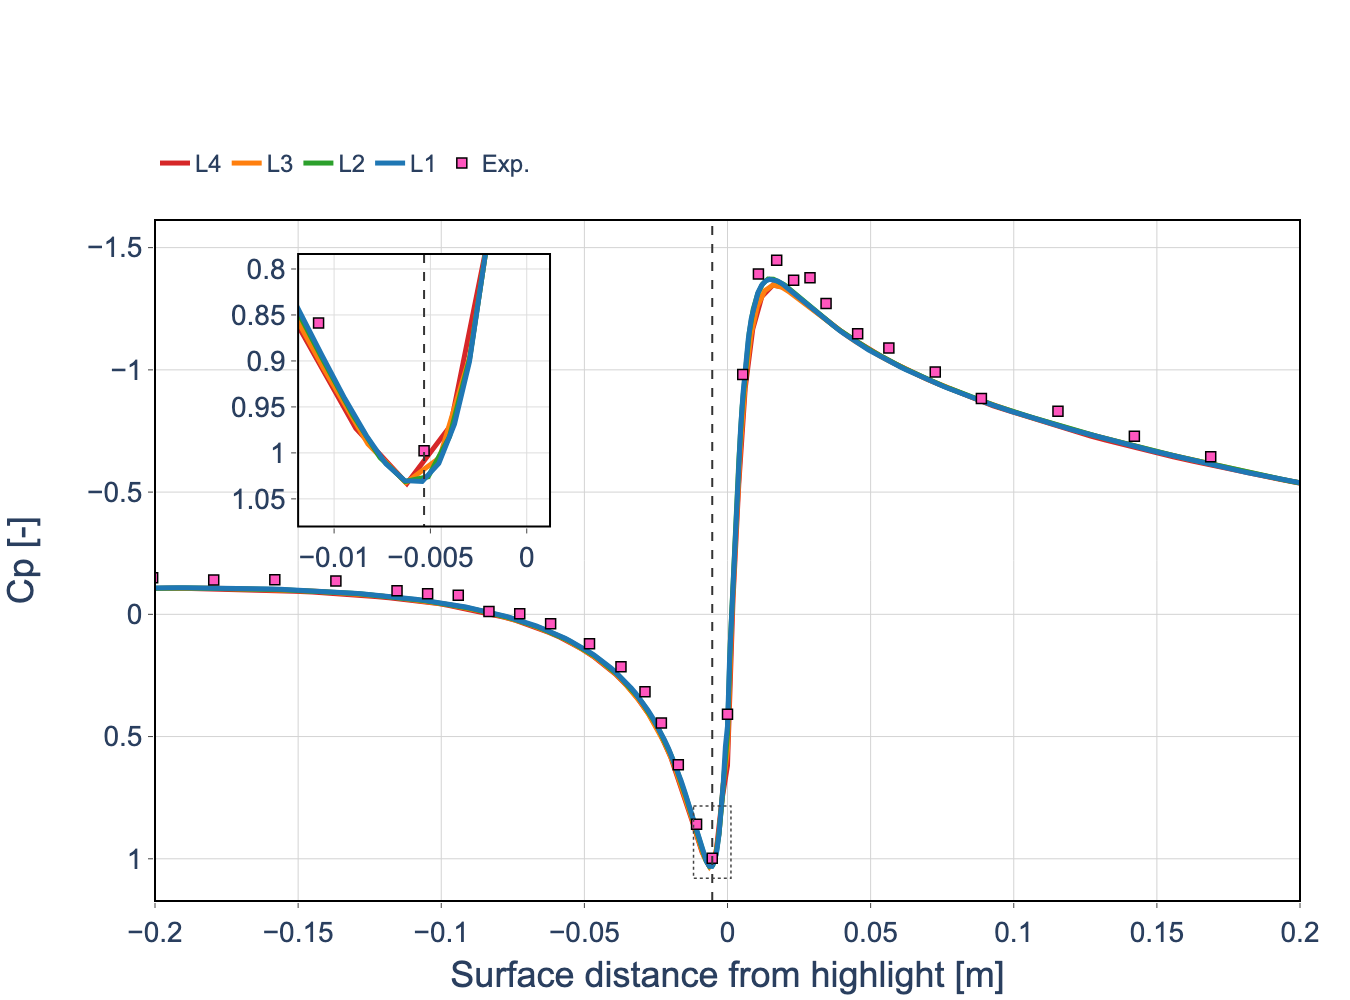
\includegraphics[
        width=\textwidth,
        trim={0cm 0cm 1cm 3.0cm},
        clip
    ]
    {FIGURES/NACA0012/AERODYNAMIC/tc_naca0012_ae3932_L1_cp_vs_s_slice_0p9144_all_roughness.png}
\end{column}

\end{columns}

\vspace{-0.05cm}

\begin{block}{\scriptsize Pressure-Coefficient Assessment}
CHAMPS predictions are in good agreement with the experimental pressure distribution across all grid levels.
\end{block}

\end{frame}


% ============================================================
% NACA0012 -- Droplet Impingement
% ============================================================

\begin{frame}{\small NACA0012 -- Droplet Impingement}
\scriptsize

\vspace{-0.15cm}

\begin{columns}[T,onlytextwidth]

% ------------------------------------------------------------
% Droplet-Bin Refinement
% ------------------------------------------------------------
\begin{column}{0.50\textwidth}
    \centering

    \textbf{Droplet-Bin Refinement -- L1, Eulerian}

    \vspace{-0.05cm}

    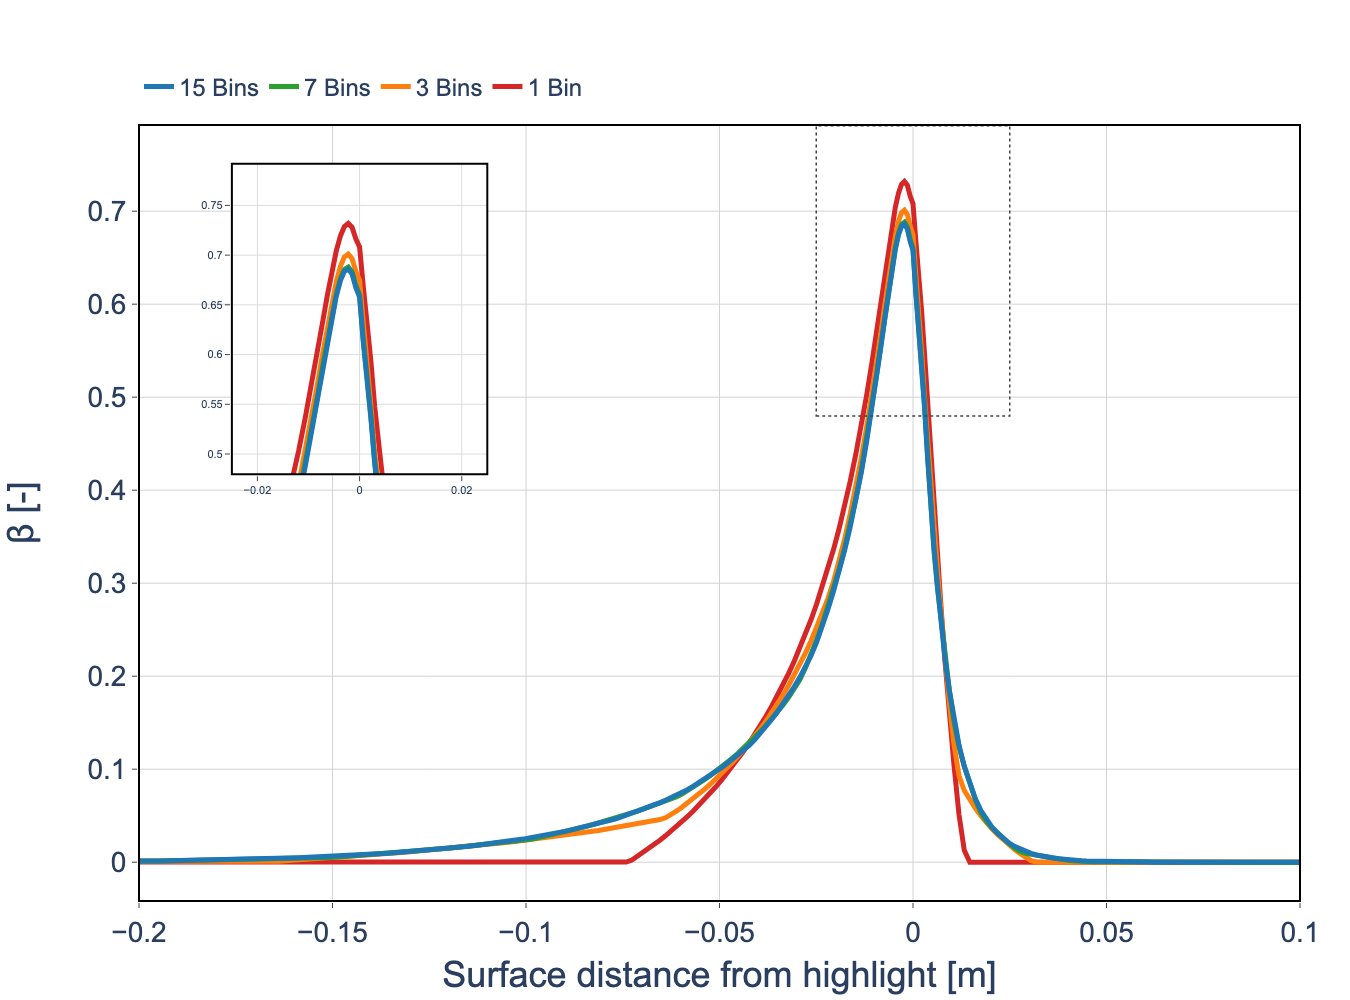
\includegraphics[
        trim={0cm 0cm 1cm 2.6cm},
        clip,
        width=\textwidth
    ]
    {FIGURES/NACA0012/IMPINGEMENT/tc_naca0012_ae3932_beta_bins07_vs_s_slice_0p9144_all_roughness_eulerian_grid_levels.png}

\end{column}

% ------------------------------------------------------------
% Eulerian vs Lagrangian
% ------------------------------------------------------------
\begin{column}{0.50\textwidth}
    \centering

    \textbf{Eulerian vs. Lagrangian -- L1, 7 Bins}

    \vspace{-0.05cm}

    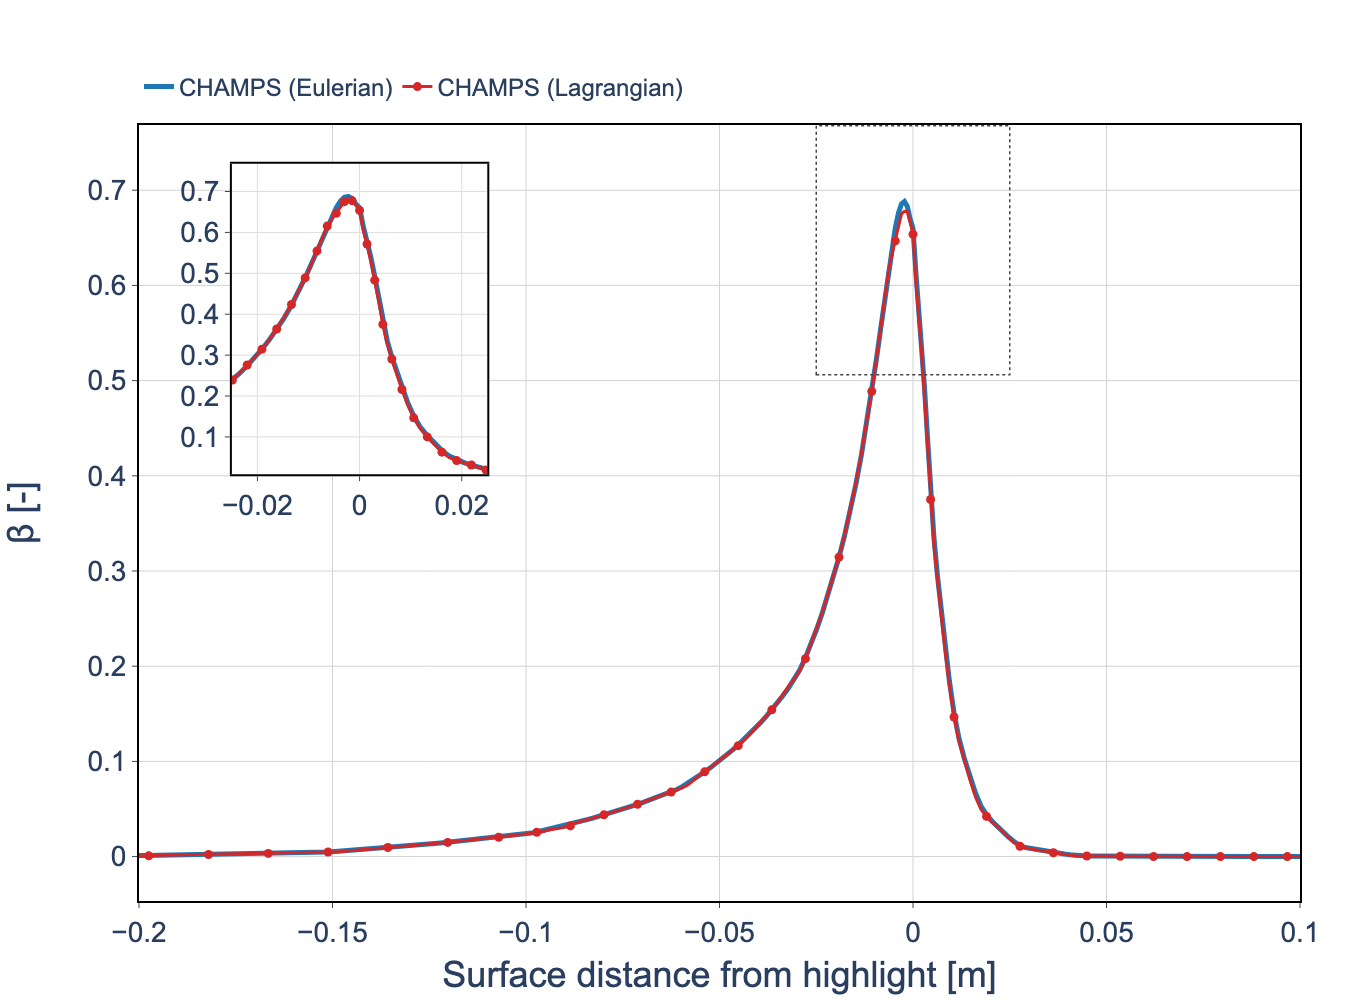
\includegraphics[
        trim={0cm 0cm 1cm 2.6cm},
        clip,
        width=\textwidth
    ]
    {FIGURES/NACA0012/IMPINGEMENT/tc_naca0012_ae3932_L1_beta_bins07_vs_s_slice_0p9144_all_roughness.png}

\end{column}

\end{columns}

\vspace{-0.15cm}

\begin{block}{\scriptsize Impingement Assessment}
\begin{itemize}
    \item Droplet-bin refinement highly affects the peak collection efficiency and impingement limits.
    \item Close agreement between the CHAMPS Eulerian and Lagrangian formulations, with minor differences near peak collection efficiency.
\end{itemize}
\end{block}

\end{frame}


% ============================================================
% NACA0012 -- Ice Mass
% ============================================================

\begin{frame}{\small NACA0012 -- Ice-Mass Prediction (15 Bins)}
\scriptsize

\vspace{-0.2cm}
\centering
% ------------------------------------------------------------
% AE3932 -- Ice Mass
% ------------------------------------------------------------
\begin{minipage}[t]{0.43\textwidth}
    \vspace{0pt}
    \centering

    \textbf{AE3932}

    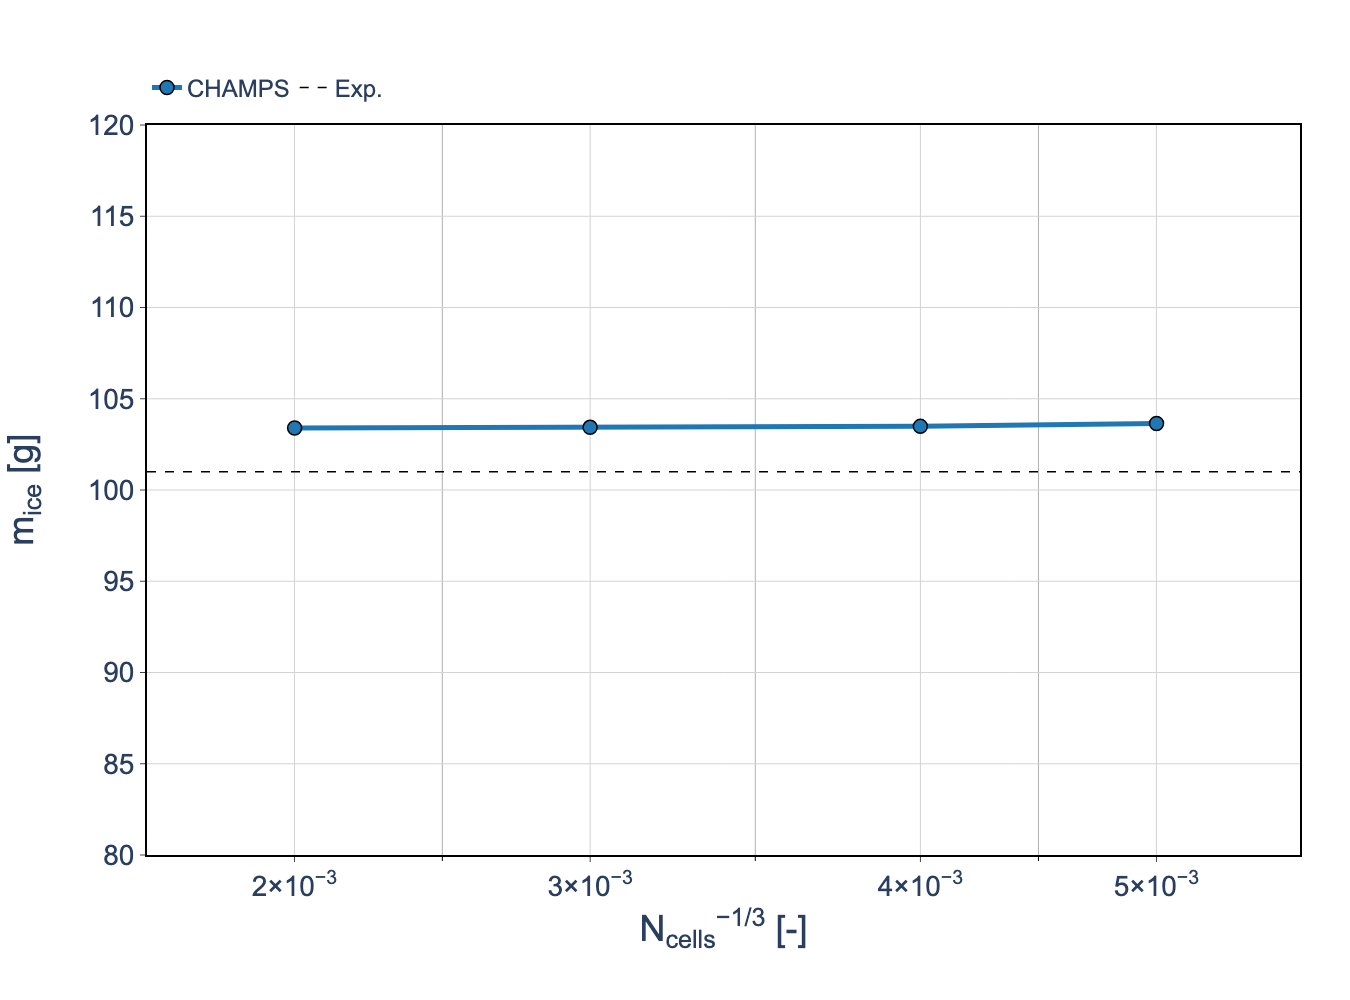
\includegraphics[
        width=\textwidth,
        trim={0cm 0cm 1cm 0.8cm},
        clip
    ]
    {FIGURES/NACA0012/ICE_ACCRETION/tc_naca0012_ae3932_ice_mass_vs_n_unspecified_bins15_all_grid_levels.png}
\end{minipage}%
\hspace{0.02\textwidth}%
% ------------------------------------------------------------
% AE3933 -- Ice Mass
% ------------------------------------------------------------
\begin{minipage}[t]{0.43\textwidth}
    \vspace{0pt}
    \centering

    \textbf{AE3933}

    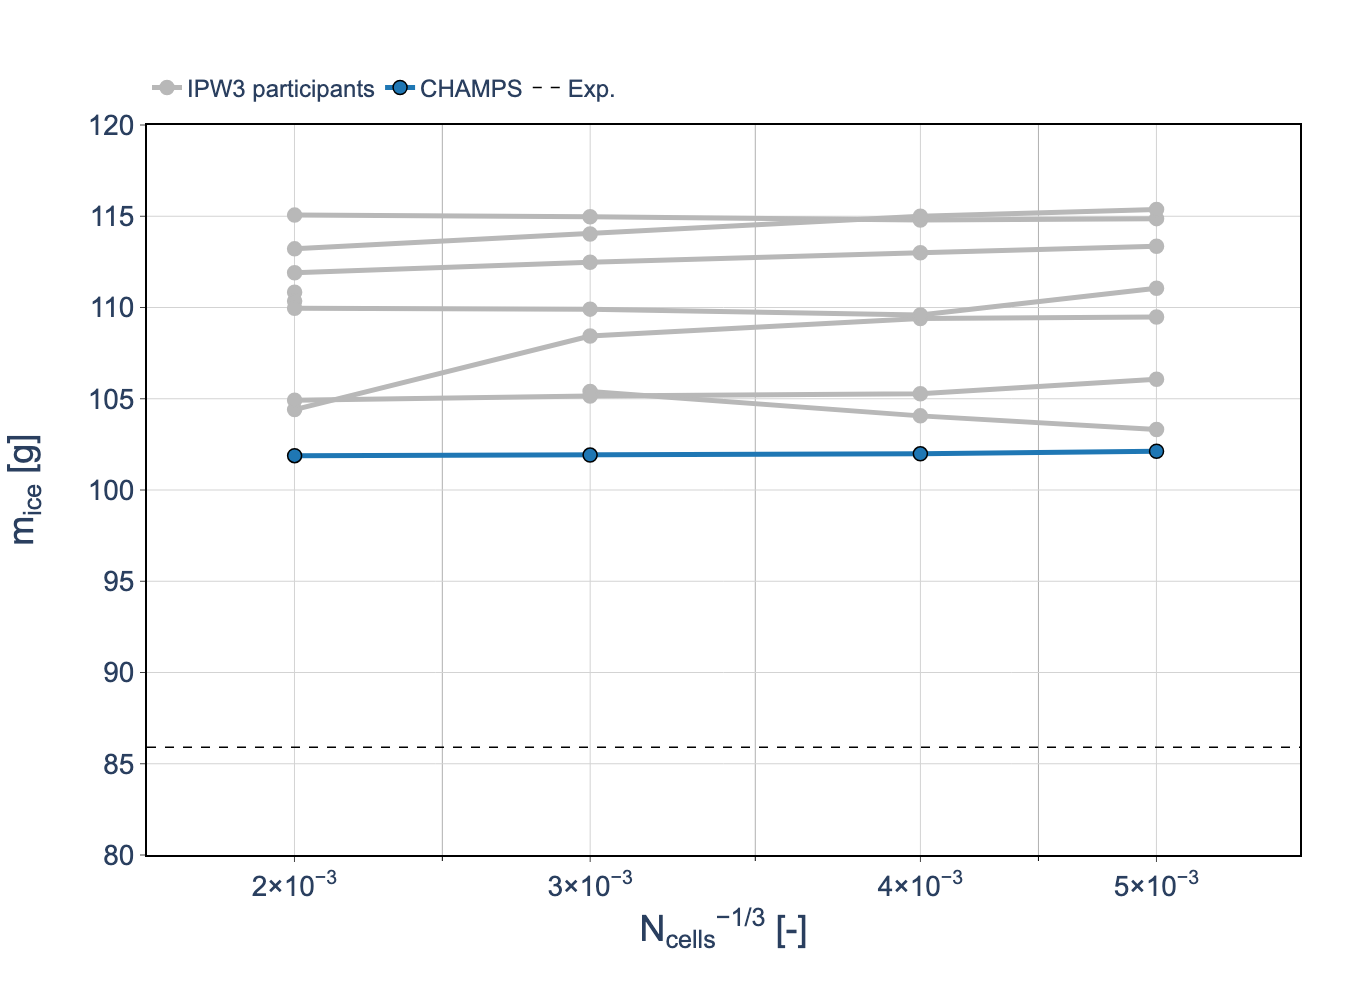
\includegraphics[
        width=\textwidth,
        trim={0cm 0cm 1cm 0.8cm},
        clip
    ]
    {FIGURES/NACA0012/ICE_ACCRETION/tc_naca0012_ae3933_ice_mass_vs_n_unspecified_bins15_all_grid_levels.png}
\end{minipage}

\vspace{-0.2cm}

% ------------------------------------------------------------
% Assessment
% ------------------------------------------------------------
\begin{block}{\scriptsize Ice-Accretion Assessment}
\begin{itemize}
    \item With the 15-bin distribution, CHAMPS predicts the AE3932 ice mass in very good agreement with the experimental value and exhibits limited sensitivity to spatial grid refinement.
    
    \item CHAMPS predicts a slightly lower ice mass for AE3933, with a reduction of approximately $1.5$ g ($\sim1.5\%$) relative to AE3932, compared with the approximately $15\%$ reduction measured experimentally.
    
    \item Approximately $88$--$90\%$ of the impinging water mass freezes into ice, with the remaining water mass lost through evaporation.
\end{itemize}
\end{block}

\end{frame}


% ============================================================
% NACA0012 -- Single-Layer Ice Shapes
% ============================================================

\begin{frame}{\small NACA0012 -- Single-Layer Ice-Shape Comparison}
\scriptsize

\vspace{-0.15cm}

\begin{columns}[T,onlytextwidth]

% ------------------------------------------------------------
% AE3932
% ------------------------------------------------------------
\begin{column}{0.50\textwidth}
    \centering
    \textbf{AE3932 - $K_s= 0.5334mm$}

    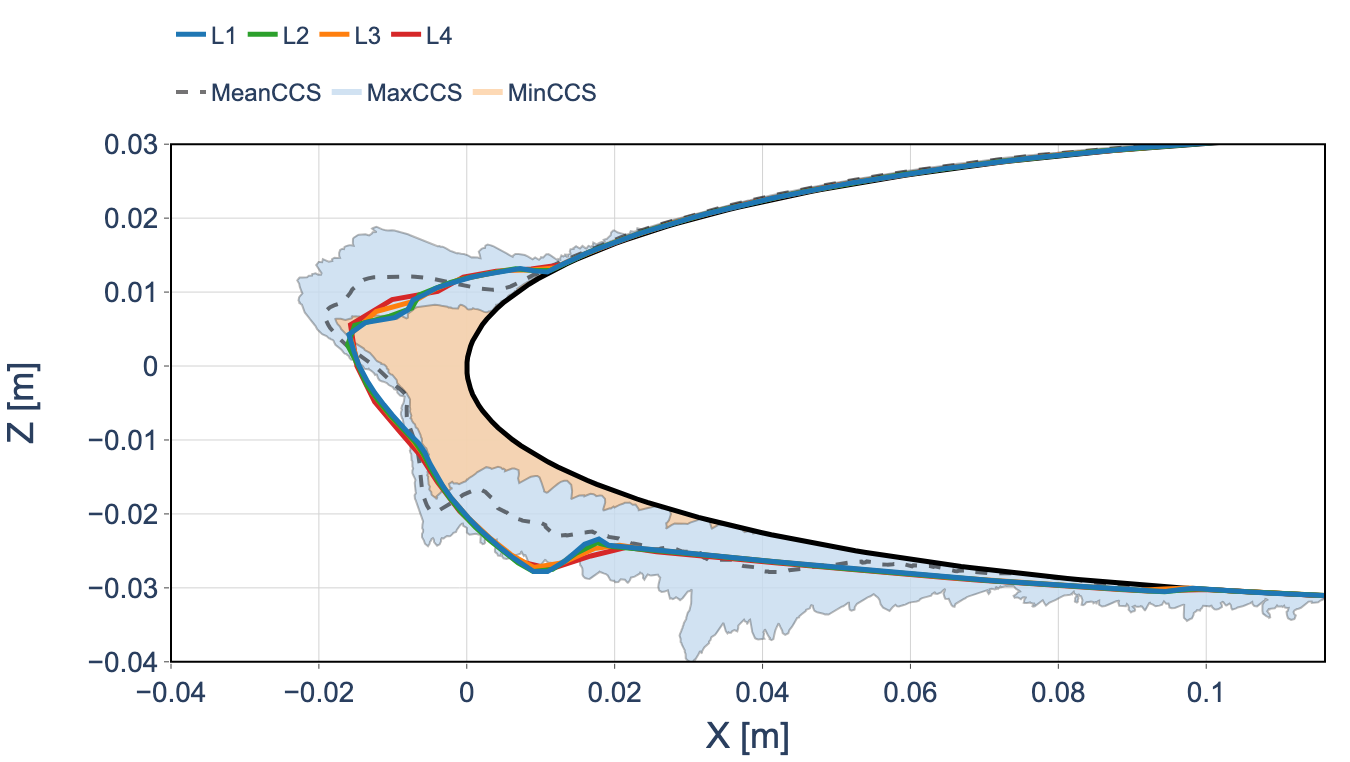
\includegraphics[
        width=\textwidth,
        trim={0cm 0cm 0cm 0.8cm},
        clip
    ]
    {FIGURES/NACA0012/ICE_SHAPES/tc_naca0012_ae3932_single_layer_ice_shape_slice_0p9144_bins15.png}
\end{column}

% ------------------------------------------------------------
% AE3933
% ------------------------------------------------------------
\begin{column}{0.50\textwidth}
    \centering
    \textbf{AE3933 - $K_s= 0.5334mm$}

    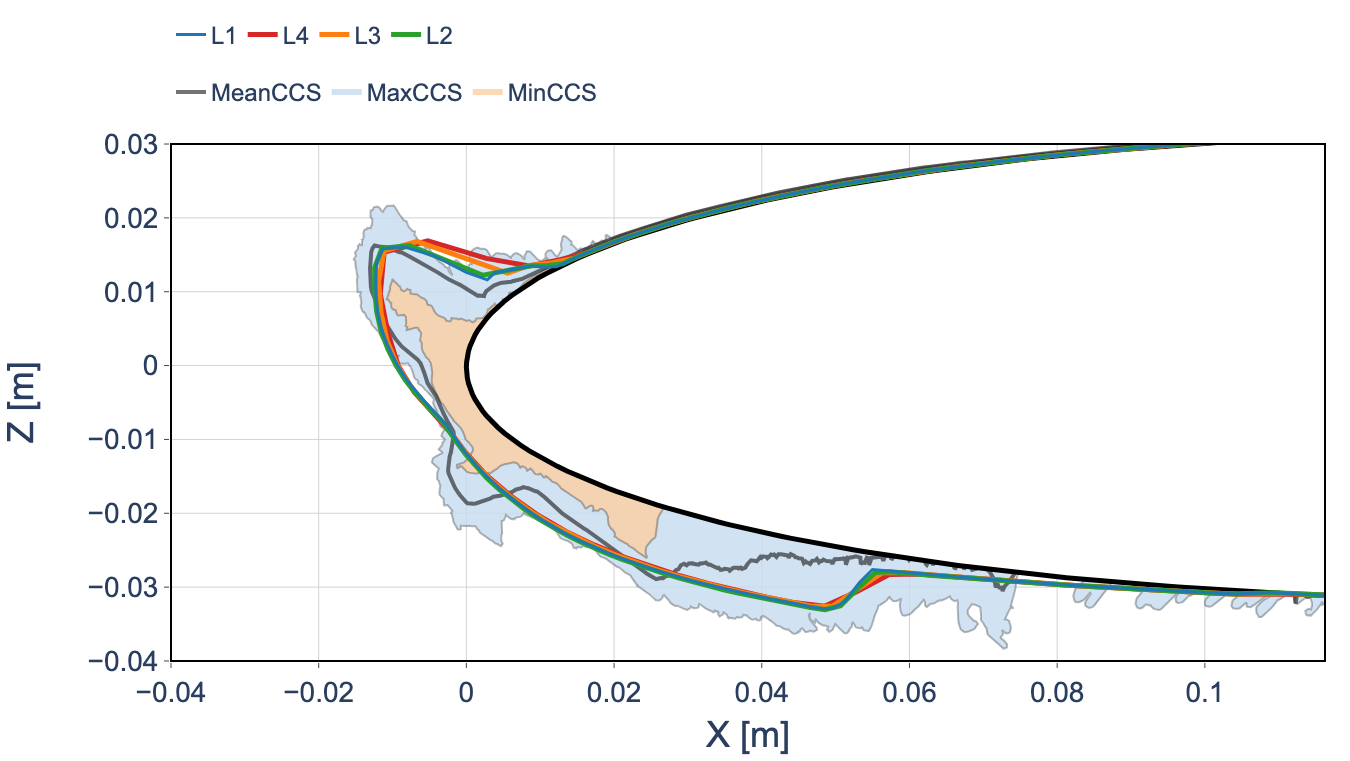
\includegraphics[
        width=\textwidth,
        trim={0cm 0cm 0cm 0.8cm},
        clip
    ]
    {FIGURES/NACA0012/ICE_SHAPES/tc_naca0012_ae3933_single_layer_ice_shape_slice_0p9144_bins15.png}
\end{column}

\end{columns}

\vspace{-0.10cm}

\begin{block}{\scriptsize Single-Layer Ice Shapes Assessment}
\begin{itemize}
    \item CHAMPS predicts consistent ice shapes across the grid hierarchy, with limited sensitivity to spatial refinement.
    \item Predictions remain largely within the experimental ice-shape envelope, with the main differences concentrated around the horn regions.
    \item Unlike the ice mass, the ice shape captures the effect of the warmer AE3933 condition, with a clear change in upper-horn orientation.
\end{itemize}
\end{block}

\end{frame}


% ============================================================
% NACA0012 -- 3D Ice Shapes
% ============================================================

\begin{frame}{\small NACA0012 -- Multilayer Ice Shapes}
\scriptsize

\vspace{-0.15cm}

\centering

% ------------------------------------------------------------
% AE3932
% ------------------------------------------------------------
\begin{minipage}[t]{0.40\textwidth}
    \centering
    \textbf{AE3932 - $K_s= 0.2667mm$}

    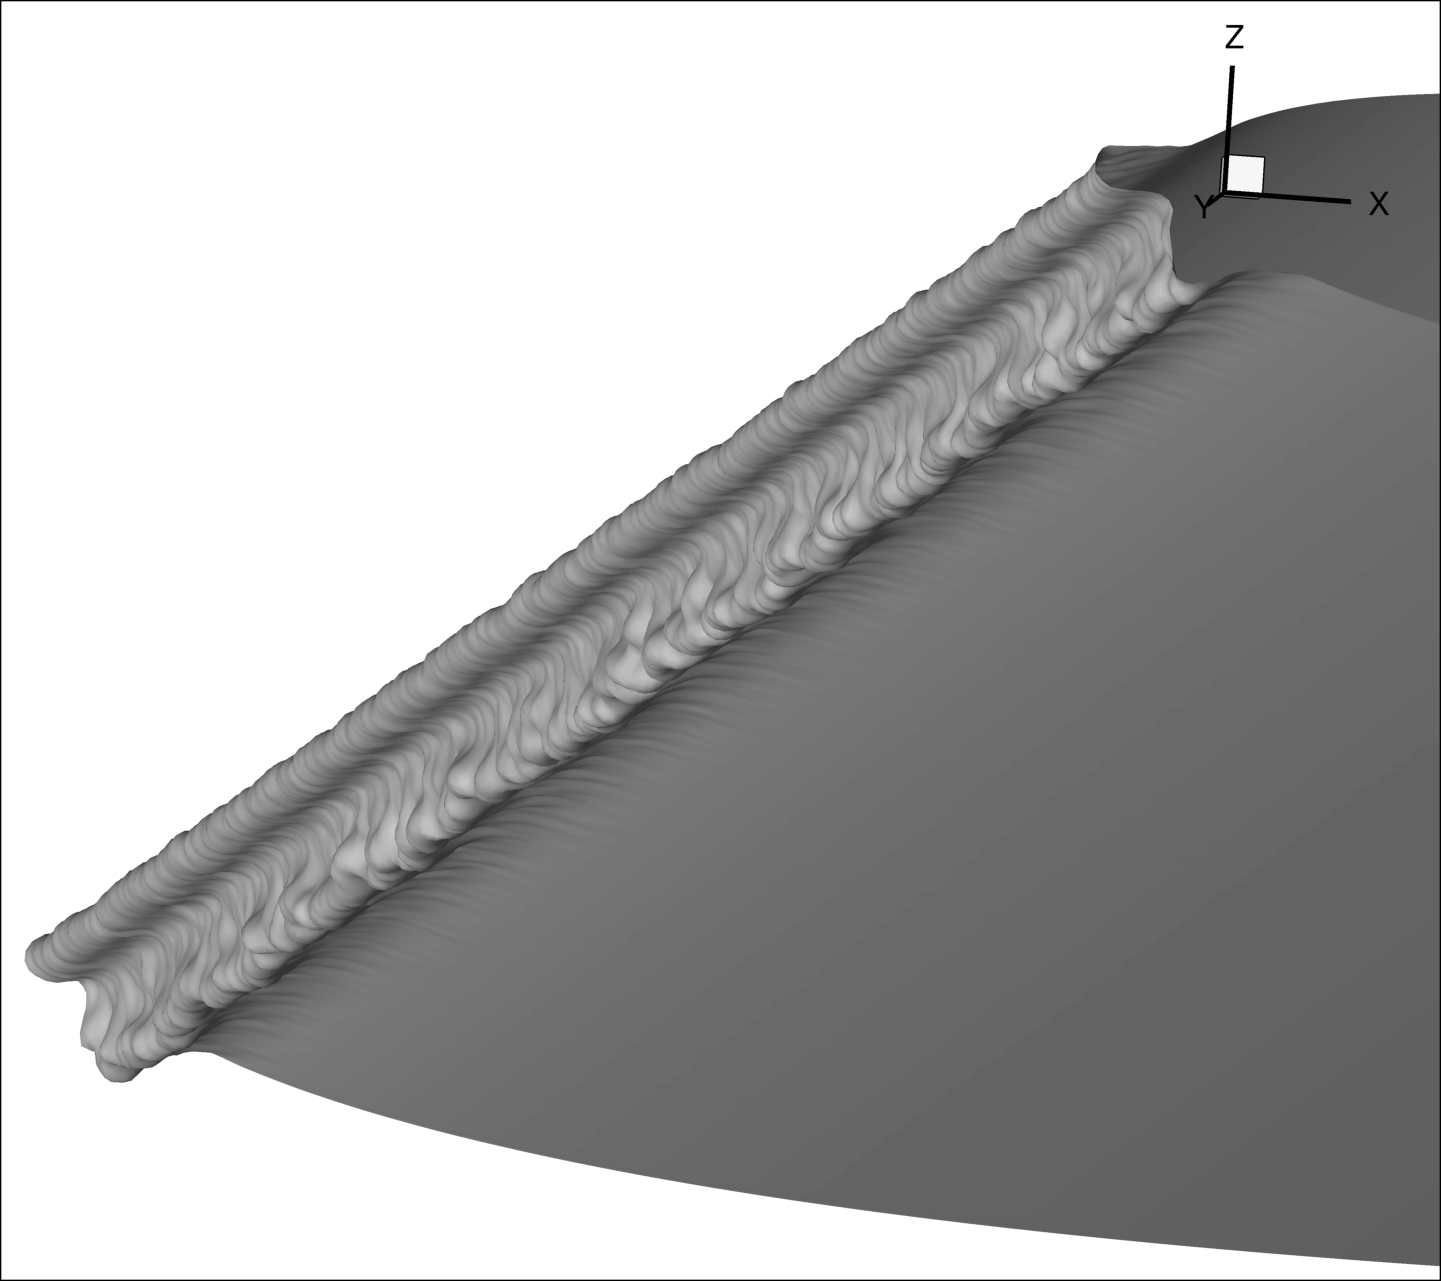
\includegraphics[
        width=\textwidth
    ]
    {FIGURES/NACA0012/ICE_VIEWS/NACA0012_AE3932.png}
\end{minipage}%
\hspace{1cm}
% ------------------------------------------------------------
% AE3933
% ------------------------------------------------------------
\begin{minipage}[t]{0.40\textwidth}
    \centering
    \textbf{AE3933 - $K_s= 0.2667mm$}

    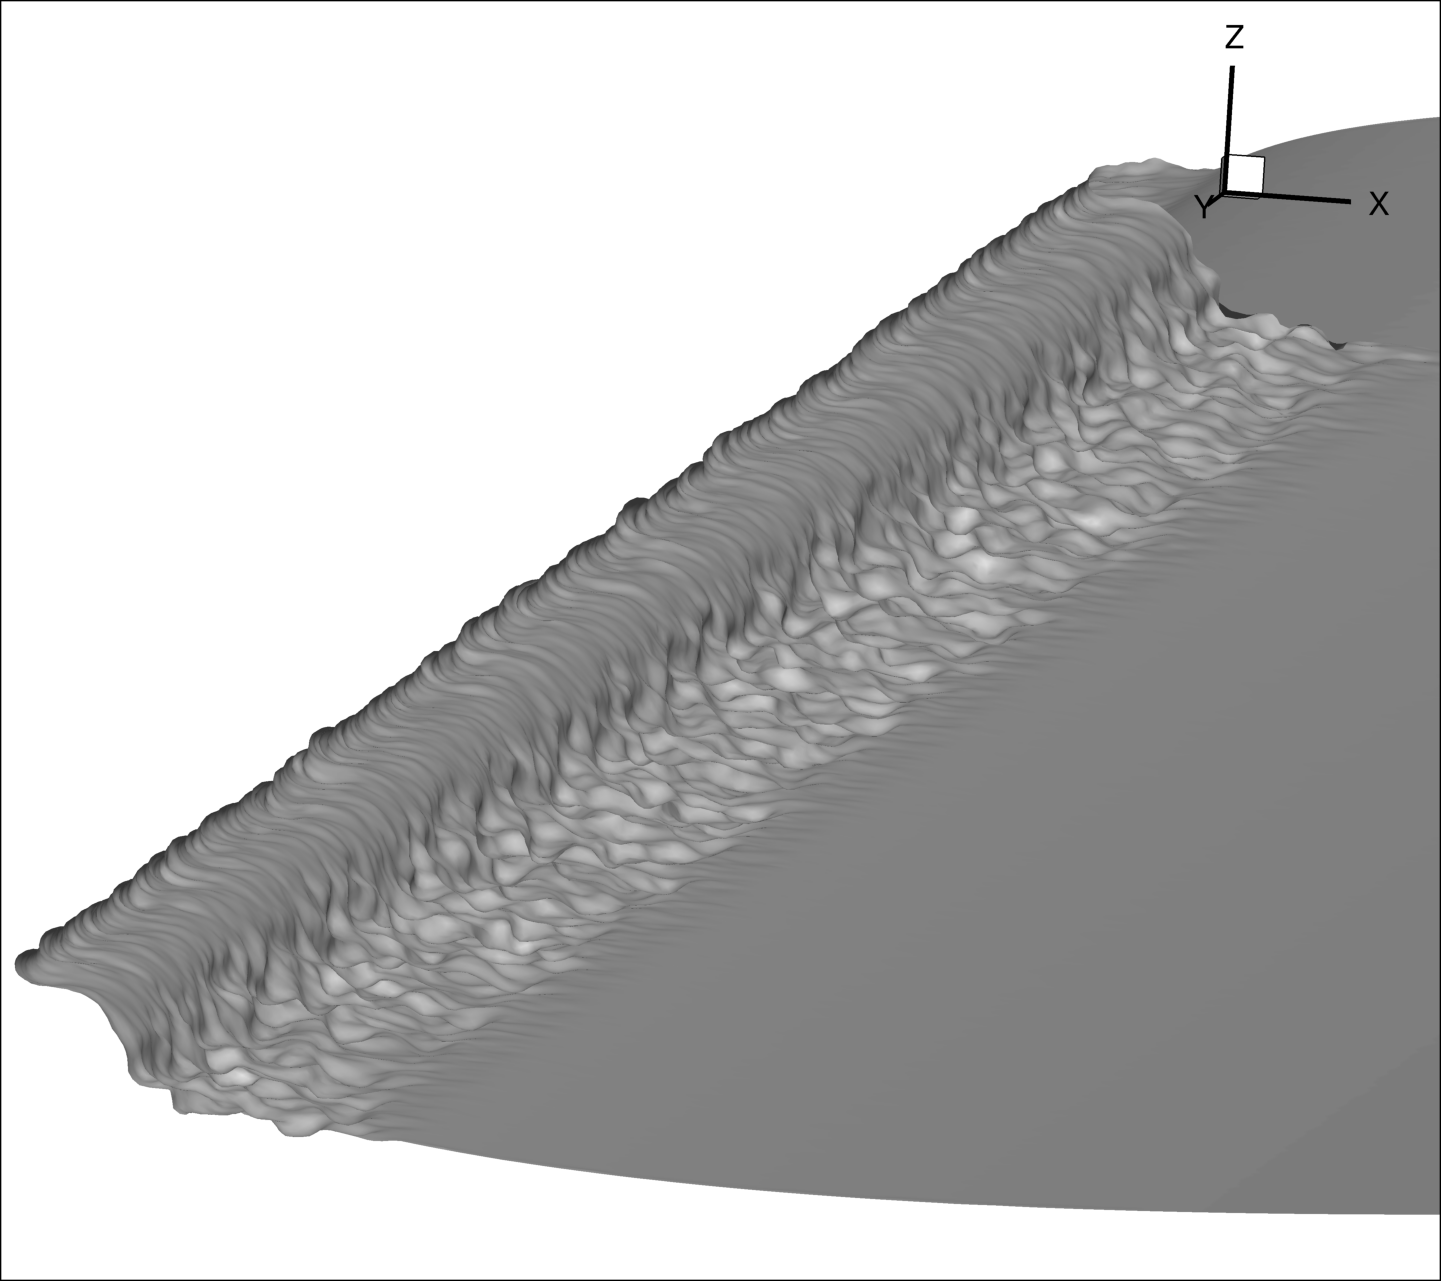
\includegraphics[
        width=\textwidth
    ]
    {FIGURES/NACA0012/ICE_VIEWS/NACA0012_AE3933.png}
\end{minipage}

\vspace{-0.10cm}

\begin{block}{\scriptsize Multilayer Ice Shapes Assessment}
\begin{itemize}
    \item The multilayer simulations capture the spanwise development of the ice horns.
    \item Distinct three-dimensional ice morphologies are obtained for the two icing conditions, consistent with the differences observed in the two-dimensional cross-sections.
\end{itemize}
\end{block}

\end{frame}


% ============================================================
% NACA0012 -- Multilayer Ice Shapes
% ============================================================

\begin{frame}{\small NACA0012 -- Multilayer Ice Shapes: Roughness Sensitivity}
\scriptsize

\vspace{-0.15cm}

\begin{columns}[T,onlytextwidth]

% ------------------------------------------------------------
% AE3932
% ------------------------------------------------------------
\begin{column}{0.50\textwidth}
    \centering
    \textbf{AE3932}

    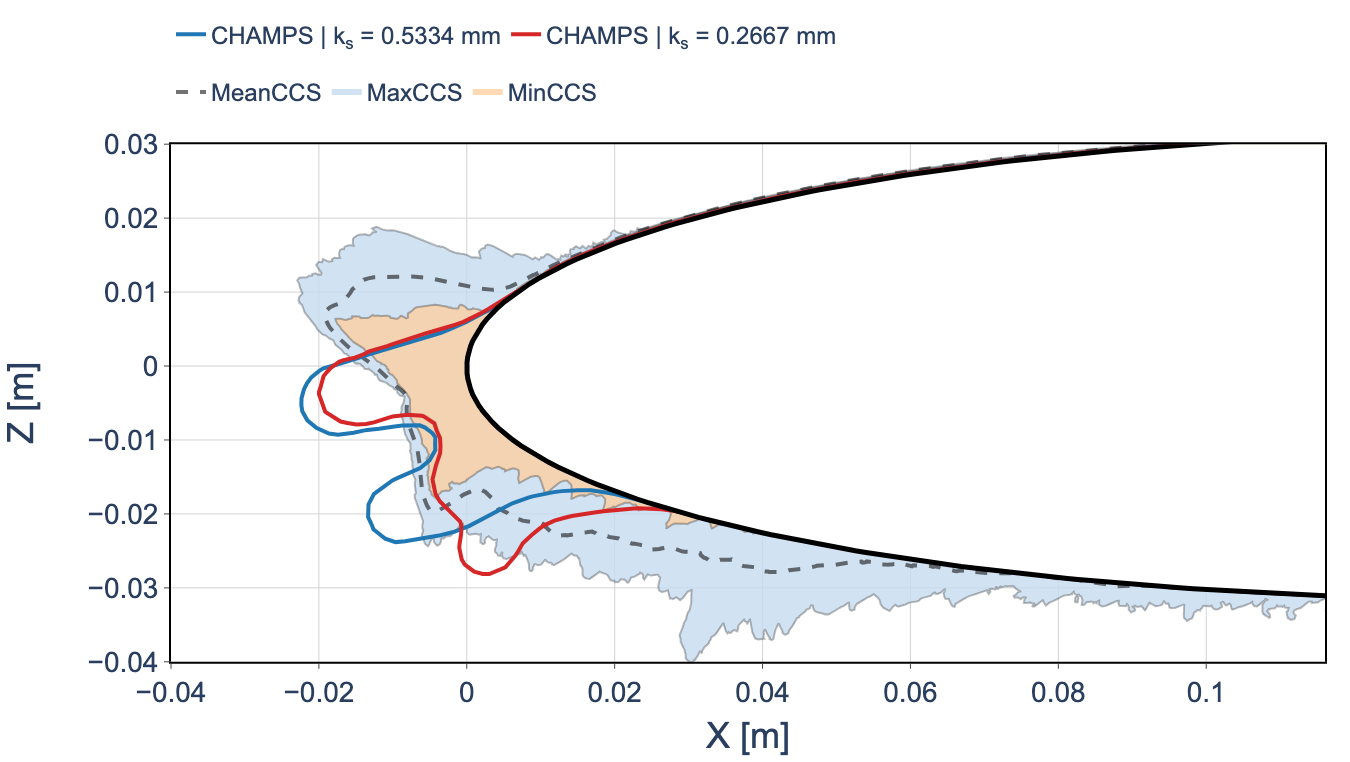
\includegraphics[
        width=\textwidth,
        trim={0cm 0cm 1cm 0.8cm},
        clip
    ]
    {FIGURES/NACA0012/ICE_SHAPES/tc_naca0012_ae3932_L1_multilayer_ice_shape_slice_0p9144_bins07_roughness_comparison.png}
\end{column}

% ------------------------------------------------------------
% AE3933
% ------------------------------------------------------------
\begin{column}{0.50\textwidth}
    \centering
    \textbf{AE3933}

    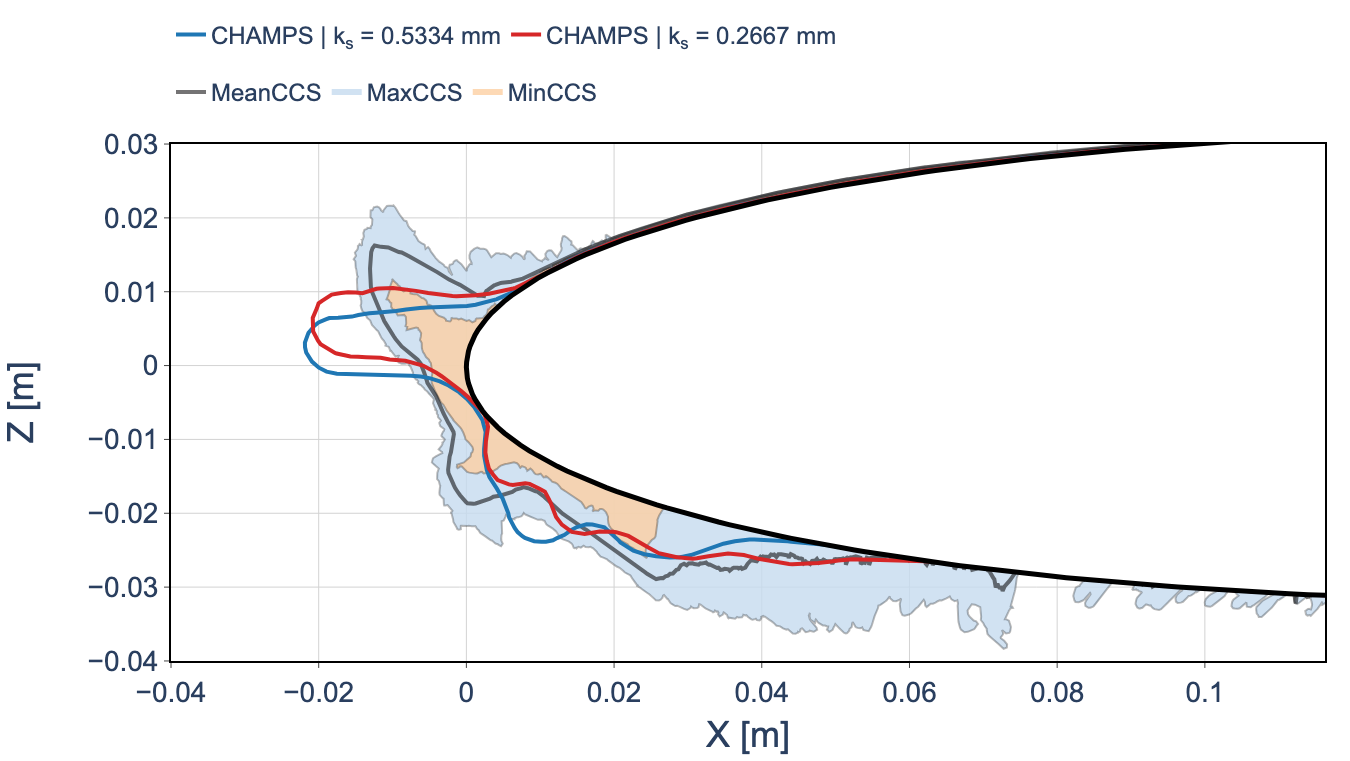
\includegraphics[
        width=\textwidth,
        trim={0cm 0cm 1cm 0.8cm},
        clip
    ]
    {FIGURES/NACA0012/ICE_SHAPES/tc_naca0012_ae3933_L1_multilayer_ice_shape_slice_0p9144_bins07_roughness_comparison.png}
\end{column}

\end{columns}

\vspace{-0.10cm}

\begin{block}{\scriptsize Multilayer Ice Shapes Assessment}
\begin{itemize}
    \item Surface roughness has a pronounced influence on the multilayer ice shapes, particularly on horn development.
    
    \item The lower roughness height provides better overall agreement with the experimental cross sections, but still underpredicts the upper-horn angle.
    
    \item The present simulations assume a constant roughness height and constant ice density, which influences the predicted location and development of the horns. Future work will investigate more advanced roughness and ice-density models for these cases.
\end{itemize}
\end{block}

\end{frame}